\chapter{Аналитический раздел}
\label{cha:analysis}

В данном разделее проведен анализ предметной области, выделены сущности протокола SMTP с точки зрения севера и их отношения.
Проведен анализ возможных схем организации рабочих процессов и сделан выбор используемой схемы.

\section{Сущности протокола SMTP на стороне сервера}

Клиент -- инициатор SMTP-сессии для передачи письма серверу в рамках его доставки от отправителя в почтовые ящики получателей.

SMTP-сессия -- процесс обмена сообщениями клиента и сервера для осуществления множества почтовых транзакции в рамках протокола SMTP, описанного в RFC 5321~\cite{RFC-5321}.

Письмо -- сообщение в формате, описанном в RFC 5322~\cite{RFC-5322}.

Почтовый ящик -- хранилище писем, имеющее адрес.

Адрес почтового ящика -- идентификатор, позволяющий однозначно определить пользователя -- получателя письма и домен сервера.

Почтовая транзакция -- операция гарантированной передачи письма без потерь данных.

Домен сервера -- идентификатор сервера.

Домен клиента -- домен сервера, с которым клиент работает в рамках одного агента доставки почты.

Отношения между сущностями представлены на рисунке~\ref{fig:er-smtp}.

\begin{figure}[ht!]
	\centering
	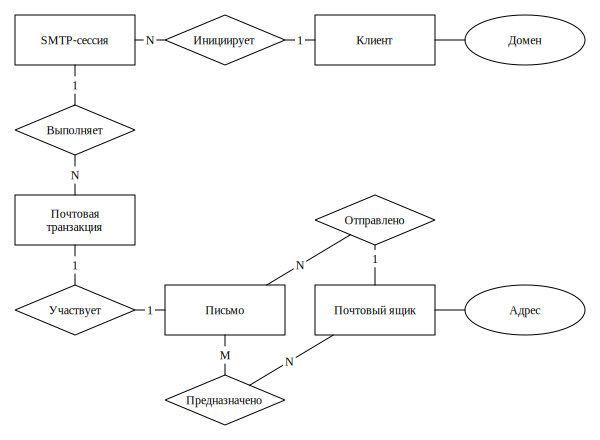
\includegraphics{inc/er-smtp.pdf}
	\caption{Модель сущностей протокола SMTP на стороне сервера}
	\label{fig:er-smtp}
\end{figure}

\section{Особенности использования системного вызова poll}

Системный вызов poll~\cite{poll} позволяет получить информацию о состоянии массива файловых дескрипторов.
Служит для обеспечения асинхронной работы с файлами, в том числе сокетами.
Является альтернативой системному вызову select~\cite{select}.
Блокирует процесс, пока не изменится состояние одного из дескрипторов.
Допускает использование таймаута.

Достоинства:
\begin{enumerate}
\item Позволяет задавать произвольное количество отслеживаемых дескрипторов.
\end{enumerate}

Недостатки:
\begin{enumerate}
\item При увеличении числа дескрипторов требуется переаллокация массива.
\item Менее переносим чем select~\cite{diff-poll-select}
\end{enumerate}

\section{Организация рабочих процессов}

В работе требуется выделить множество рабочих процессов, ослуживающих соединения.
Существует несколько подходов.

\subsection{Множество равнозначных процессов}

Процесс создает неблокирующий слушающий сокет, выполняя цепочку системных вызовов: socket, bind, listen.
Затем создает клонов c помощью системного вызова fork, каждый из которых, в том числе первый процесс (можно и без него) вызывает poll для слушающего и множества клиентских сокетов.
При возникновении события на слушающем сокете выполняется системный вызов accept.
Гарантируется, что только одному процессу вернется дескриптор клиентского сокета.
В других accept завершится с ошибкой.

Достоинства:
\begin{enumerate}
\item Один алгоритм работы процессов.
\item Отсутствие накладных расходов для начала обслуживания клиентского сокета.
\end{enumerate}

Недостатки:
\begin{enumerate}
\item Отсутствие планировщика, распределяющего нагрузку.
\item Отсутствие возможности получать информацию о состоянии других процессов без накладных расходов.
\item Конкуренция на слушающем сокете.
\item Крах одного процесса ведет к понижению производительности системы с невозможнотью восстановления без полного перезапуска.
\end{enumerate}

\subsection{Централизованная схема}

Главный процесс создает блокирующий слушающий сокет, выполняя цепочку системных вызовов: socket, bind, listen.
Затем создает подчиненные процессы c помощью fork, устанавливая с ними соединение через Unix-сокет.
Далее в цикле вызывает accept.
Клиентский сокет отправляется подчиненному процессу в соответсвии с алгоритмом распределения нагрузки.
Если соединение с подчиненным неожиданно закрылось, можно завершить подчиненный процесс и создать новый вместо него.
Подчиненный процесс вызывает poll для сокета соединения с главным и множества клиентских сокетов.
Клиентские сокеты получаются через соединение с главным процессом.

Достоинства:
\begin{enumerate}
\item Отсутствие конкуренции на слушающем сокете.
\item Возможность получения состояния подчиненного процесса.
\item Крах подчиненного процесса не ведет к краху системы.
\end{enumerate}

Недостатки:
\begin{enumerate}
\item Крах главного процесса потребует перезапуска всех процессов.
\item Два алгоритма работы.
\item Накладные расходы для начала обслуживания клиентского сокета.
\end{enumerate}

\subsection{Схема <<ведущий-ведомый>>}

Аналогична централизованной схеме, только подчиненные процессы -- ведомые между собой имеют соединение.
В случае краха главного процесса -- ведущего при наличии кворума выбирается новый ведущий, который восстанавливает систему.

Достоинства:
\begin{enumerate}
\item Отсутствие конкуренции на слушающем сокете.
\item Получение состояния ведомых процесса без накладных расходов.
\item Крах любого из процессов не ведет к краху системы.
\end{enumerate}

Недостатки:
\begin{enumerate}
\item Множество нетривиальных алгоритмов работы.
\item Большие накладный расходы на взаимодействие между процессами.
\item Накладные расходы для начала обслуживания клиентского сокета.
\end{enumerate}

\subsection{Используемая схема организации работы процессов}

В рамках данной работы будет использована централизованная схема.
Во-первых, ввиду отсутствия конкуренции за ресурсы
Во-вторых, отказоустойчивости процессов, обслуживающих клиентов.
Вероятность краха подчиненных процессов значительно выше вероятности краха главного, в соответствии с разницей в сложности алгоритмов.
Такая схема позволяет более детально изучить межпроцессное взаимодействие.
Распределение клиентских сокетов будет выполняться циклическим алгоритмом.
